\documentclass[11pt]{article}
\usepackage{amsmath}
\usepackage{amsfonts}
\usepackage{amssymb}
\usepackage{xspace}

\usepackage{caption}
\usepackage{subcaption}

\usepackage{hyperref}


% \newcommand{\eg}{\textit{eg.}}
% \newcommand{\ie}{\textit{i.e.}}

\newcommand{\ks}[1]{\textcolor{red}{[KS: #1]}}

\newcommand{\D}{\text{d}\xspace}

\newcommand{\xbf}{\mathbf{x}\xspace}
\newcommand{\abf}{\mathbf{a}\xspace}
\newcommand{\cbf}{\mathbf{c}\xspace}
\newcommand{\fbf}{\mathbf{f}\xspace}
\newcommand{\ebf}{\mathbf{e}\xspace}
\newcommand{\wbf}{\mathbf{w}\xspace}
\newcommand{\vbf}{\mathbf{v}\xspace}
\newcommand{\ubf}{\mathbf{u}\xspace}
\newcommand{\sbf}{\mathbf{s}\xspace}
\newcommand{\Sbf}{\mathbf{S}\xspace}
\newcommand{\Xbf}{\mathbf{X}\xspace}
\newcommand{\Zbf}{\mathbf{Z}\xspace}
\newcommand{\zbf}{\mathbf{z}\xspace}
\newcommand{\ybf}{\mathbf{y}\xspace}
\newcommand{\dbf}{\mathbf{d}\xspace}
\newcommand{\bbf}{\mathbf{b}\xspace}
\newcommand{\mbf}{\mathbf{m}\xspace}

\newcommand{\onebf}{\mathbf{1}\xspace}
\newcommand{\zerobf}{\mathbf{0}\xspace}
\newcommand{\threebf}{\mathbf{3}\xspace}

\newcommand{\Gbf}{\mathbf{G}\xspace}
\newcommand{\Abf}{\mathbf{A}\xspace}
\newcommand{\Bbf}{\mathbf{B}\xspace}
\newcommand{\Ubf}{\mathbf{U}\xspace}
\newcommand{\Vbf}{\mathbf{V}\xspace}
\newcommand{\Dbf}{\mathbf{D}\xspace}
\newcommand{\Ebf}{\mathbf{E}\xspace}
\newcommand{\Qbf}{\mathbf{Q}\xspace}
\newcommand{\Lbf}{\mathbf{L}\xspace}
\newcommand{\Ibf}{\mathbf{I}\xspace}
\newcommand{\Mbf}{\mathbf{M}\xspace}

\newcommand{\Lambdabf}{\bm{\Lambda}\xspace}
\newcommand{\lambdabf}{\bm{\lambda}\xspace}
\newcommand{\mubf}{\bm{\mu}\xspace}
\newcommand{\epsbf}{\bm{\epsilon}\xspace}
\newcommand{\Sigmabf}{\bm{\Sigma}\xspace}
\newcommand{\Thetabf}{\bm{\Theta}\xspace}
\newcommand{\one}{\mathds{1}\xspace}
\newcommand{\trace}{\text{tr}\xspace}


\newcommand{\CG}{G\xspace}
\newcommand{\CV}{V\xspace}
\newcommand{\CT}{\mathcal{T}\xspace}
\newcommand{\CE}{E\xspace}
\newcommand{\CA}{\mathcal{A}\xspace}
\newcommand{\CB}{\mathcal{B}\xspace}
\newcommand{\CD}{\mathcal{D}\xspace}
\newcommand{\CX}{\mathcal{X}\xspace}
\newcommand{\CY}{\mathcal{Y}\xspace}
\newcommand{\CK}{\mathcal{K}\xspace}
\newcommand{\CM}{\mathcal{M}\xspace}
\newcommand{\CC}{\mathcal{C}\xspace}
\newcommand{\CL}{\mathcal{L}\xspace}
\newcommand{\CI}{\mathcal{I}\xspace}

\newcommand{\Mod}[1]{\ (\mathrm{mod}\ #1)}

\newtheorem{prob}{Problem}

\begin{document}

\title{Limitations of low dimensional graph embeddings}

\author{C. Seshadhri\footnote{University of California, Santa Cruz. {\tt sesh@ucsc.edu}. Supported by NSF DMS-2023495, CCF-1740850, 1839317, 1908384}}

\date{}
\maketitle
\renewcommand\thesection{\arabic{section}}
\setcounter{section}{0}
\setcounter{figure}{0}
\setcounter{table}{0}

\begin{abstract}
The learning of graph representations, also called graph embeddings, is a fundamental technique in machine learning (ML).
The aim is to represent the vertices of a graph by low-dimensional real-valued vectors, which can be 
used for a variety of downstream ML tasks. The popular technique of Graph Neural Networks (GNNs) can
be thought of a type of graph representation learning method. This article surveys some recent work on the \emph{limitations}
of graph embedding methods. These results provide mathematical theorems proving that low-dimensional
embeddings cannot recreate ``community-like" structure, through commonly used kernels. These theorems
are supported by empirical results, showing that many classic graph embedding methods actually perform
poorly on important machine learning tasks. Low-dimensional representations often lose
much of the fine-grained community structure of real-world data. The results surveyed in this article
provide an interesting counterpoint to the popularity of graph embeddings and GNNs for machine learning.
\end{abstract}

\section{Introduction}

Capturing the rich structure of graph is central for many machine learning tasks.
The heterogenous, non-local, and massive structure
of modern graphs are a problem for many basic machine learning tasks,
such as ranking, link prediction, and classification~\cite{easley2010networks}.
\emph{Graph representation learning} provides a
convenient solution to this problem. Each vertex
of a graph is represented as a vector in low-dimensional space. 
These vectors form the (low-dimensional) embedding of the graph.
The vectors can be used for a plethora of downstream machine learning tasks.
The aim is to have these vectors combine the graph structure with vertex features into
a compact geometric representation.

The study of low-dimensional graph embeddings is an incredibly popular
research area, and has generated many exciting results over the past
few years (see surveys~\cite{HaYiLe18, MLGSurvey20} and a Chapter 23 in~\cite{pml1Book}). 
The most successful methods for graph embeddings often use Deep Learning techniques,
together with classic approaches like matrix factorization~\cite{PeAlSk14,GrLe16,OuCu16,PeKu+17,QiDo18,LiWu19}. Graph Neural Networks (GNNs)
can be thought of as specific class of graph embeddings algorithms~\cite{HaYiLe17,VeCu+18,XuHuLe+19}.
Despite the large variety of algorithms used for graph representation learning (and specifically GNNs),
their output has a simple, consistent structure. Given a graph $G$ on $n$
vertices, these methods map each vertex to a vector in $\sRR^d$, where
$d \ll n$. In a typical applications, $n$ is the order of millions or more,
while $d$ is in the hundreds.

Much of the advances in this field are primarily empirical; there
are numerous papers in major machine learning conferences on more
complex GNN architectures or more involved graph embedding methods.
Nonetheless, there is limited principled understanding of the power of low-dimensional
graph embeddings. Small changes in training or input data can lead to major differences
in the output~\cite{GuVi+19}. Much of the research on graph embeddings and GNNs, for example, report significant success in prediction
tasks on graphs~\cite{GrLe16,HaYiLe17,QiDo18}. On the other hand, some papers suggest that low-dimensional graph embeddings
can be beaten by simpler hand-tuned methods~\cite{GuVi+19,HuHe+21}.
It is useful to have a rigorous mathematical framework to understand graph embeddings.
Specially, we wish to address the following questions.

\begin{asparaitem}
    \item To what extent can relevant graph structure be captured by low-dimensional graph embeddings?
    \item How does low-dimensional geometry relate to downstream ML tasks on graphs?
    \item How does the choice of kernel functions (for prediction tasks) affect the task?
\end{asparaitem}

\medskip

Contrary to most research in this area, our approach to investigating these questions is through \emph{limitations}
or lower bounds. Our aim is develop a theoretical framework that is agnostic to the specific
algorithm performing the embedding. We first describe some basic terminology and central concepts.

\paragraph{The importance of matrix factorizations:} A low-dimensional matrix factorization approximates
gives an algorithm-independent view of how low-dimensional embeddings represent graphs. We think
of $M$ as an adjacency matrix, or any matrix representation of our graph $G$. In many Deep Learning
methods, $M$ is constructed by long walks with appropriate vertex-centric aggregation functions~\cite{PeAlSk14,GrLe16,PeKu+17}.
The matrix $V$ is the collection of embeddings, where each column vector corresponds to a vertex.
Recent work has shown the many different graph embedding methods can be cast as matrix factorizations,
with different choices of matrices $M$, and different notions of approximations~\cite{QiDo18}. Indeed, the simplest
low-dimensional embedding is obtained by a low-rank SVD of the adjacency matrix, arguably the most
basic of matrix factorizations.

\medskip

\paragraph{The importance of dot products:} Regardless of how the graph embedding vectors are obtained,
the general strategy is to use ``nearness" in geometric space as a proxy for the similarity of the corresponding
vectors. Thus, the downstream ML tasks treat vertices $i$ and $j$ as similar if their corresponding
vectors $\vec{v}_i$ and $\vec{v}_j$ are similar. Arguably, the most important measure of similarity is 
the dot product $\vec{v}_i \cdot \vec{v}_j$ or cosine similarity (which is a normalized dot product). 
This has special significance for matrix factorizations,
since $V^TV$ is precisely the matrix of all pairs of dot products.

Even when the embedding vectors are not obtained by matrix factorizations, the Gram
matrix $V^TV$ is commonly used for downstream prediction tasks. A natural strategy for any prediction task 
is to use nearest neighbor (k-NN) search according to the dot product/cosine similarity. There are many open course packages for k-NN, making it 
the default choice in industrial applications of graph embeddings~\cite{Sci}. 

\medskip

We now can formalize our initial questions in matrix language. 
Observe how there is no reference to any embedding method or GNN;
we directly analyze the behavior of the output representation.

\begin{center}
Can a Gram matrix $V^TV$ for $V \in \sRR^{d \times n}$ ($d \ll n$)
capture the structure of either real-world networks
or the properties of prediction matrices arising from downstream ML tasks
(on graphs)?
\end{center}

This framework captures the vast majority of graph embedding constructions and applications.

\subsection{Limitations of graph embeddings} \label{sec:limit}

This article presents two results on the limitations of low-dimensional graph embeddings
for prediction and machine learning on real-world graphs~\cite{SeSh20,StLe+22}. The underlying
theoretical results are algorithm agnostic, and the limitations hold for \emph{any} graph embedding
algorithm. These results come with empirical backing, performed on classic and important graph
embedding methods.

\paragraph{Inability to recreate triangle structure~\cite{SeSh20}:} This result focuses
on the fundamental premise of low-dimensional embeddings, rather than a specific ML task. 
Algorithms to construct (or predict from) low-dimensional embeddings implicitly pose
a low-dimensional graph/matrix model. This model represents a distribution of graphs
that are created from a set of real vectors (where each vector represents a vertex). The embedding
is constructed by fitting this model to an input graph, typically using dot product as a 
proximity measure.

This result mathematically proves that no low-dimensional model (using a dot product kernel) can simultaneously
recreate two central properties of real-world graphs: sparsity and triangle density. It is well-known
from the early days of network science that real-world graphs are sparse but have high clustering
coefficients~\cite{WaSt98,SaCaWi+10,SeKoPi12,DuPi+12}. Hence, typical models used to construct low-dimensional embeddings cannot
generate realistic graphs. They miss the (crucial) triangle structure of real data.

The theory is supported with empirical results. These empirical results are demonstrated
on other kernels beyond the dot product, thus suggesting that the limitations are fundamental.
We discuss these results in \Sec{imp-tri}.

There are notable counterpoints to these results.
Firstly, Chanpuriya et al show that asymmetric embeddings avoid the rank lower bounds
discussed above~\cite{CMST20}. Another result of Chanpuriya et al shows that graphs can sometimes be
reconstructed from their embeddings. In some cases, the community structure of the reconstruction
is actually enhanced~\cite{ChMu+21}. We give more detail in \Sec{imp-tri}.

\paragraph{Weak performance on community labeling tasks~\cite{StLe+22}:} This result takes
a complementary angle, and focuses on a downstream ML task. Community labeling is a binary
prediction problem, where we wish to predict if two vertices belong to a community.
This work sets up a community labeling problem for both real and synthetic data sets. First,
the authors create a simple benchmark algorithm using logistic regression on classic graph 
features (like Personalized PageRank and short path counts). This benchmark has fairly
good performance, as measured by distributions of local precision. On the other hand,
many well-established graph embedding methods have surprisingly poor performance
on the same task.

These observations are backed up with theoretical proofs. The prediction matrices
based on low-dimensional embeddings provably do not have the typical community
structure of real data. This work also investigates alternate kernels,
like the normalized softmax (used in results like {\tt DeepWalk} and {\tt node2vec}~\cite{PeAlSk14,GrLe16}).
These kernels have other limitations in that slight noise can destroy community
structure in the corresponding prediction matrices.

These results are discussed in \Sec{poor-comm}.

\subsection{Broader context} \label{sec:context}

A reader may ask: how are the limitations stated in this article consistent
with large body of work on the effectiveness of graph embeddings and GNNs?
Our answer is two-fold, backed up by~\cite{GuVi+19,HuHe+21}. First, most research on graph embeddings compare various representation
learning methods with each other, and do not consider alternative baselines. Secondly, we believe that many graph embeddings methods do not 
have good predictions with respect to other metrics. For example, almost all
these result use the AUC metric to measure link prediction performance. On the other hand,
AUC is a bad measure for sparse ground truth~\cite{Ha09,LiCh12}. Indeed, in \Sec{poor-comm},
we show poor prediction performance (for graph embedding methods) on a local precision metric.

There has been compelling empirical work showing that GNNs and embeddings can be 
outperformed by simpler methods. We mention two results in detail because
they highlight empirical weaknesses in graph embeddings, and reinforce the
previous points.

{\bf Gurukar et al, the lack of good experimental design~\cite{GuVi+19}:} Gurukar et al do a detailed comparison of twelve
different graph representation learning methods on a variety of ML tasks. They focus on two
of the most important tasks of link prediction and node classification. Despite
there being many newer methods, they observe that the {\tt M-NMF} algorithm
is best for link prediction~\cite{WaCu+17} and {\tt NetMF} algorithm~\cite{QiDo18} is best for node classification.
No graph representation method outperforms on both metrics. This paper does an exceptional
job of clearly specifying the experimental design and thoroughly investigating previous work.

Along the lines of the current article, simple task specific baselines are competitive with
graph embedding methods. These baselines are formed by a simple model that uses basic graph features
(like Common Neighbors, Adamic-Adar index~\cite{AdAd03}, Jaccard similarity, etc.). These results
are analogous to what we observe in~\cite{StLe+22}. 

Gurukar et al point out a major problem with evaluations in graph embedding papers.
Quoting from there: ``$\ldots$ a new method
almost always compares its performance against a subset of
other methods [and] datasets previously evaluated. While great care is taken
to tune the new method, the same care is often not taken when evaluating baselines."

{\bf Huang et al, easier methods beat GNNs~\cite{HuHe+21}:} Huang et al devise
an alternate graph learning algorithm called \emph{Correct and Smooth (C\&S)}.
Consider the problem of node classification. This method starts with a ``base predictor"
that ignores the graph structure. Using only node features, one can train
a basic model for classification. Then, the graph is introduced a post-processing
step to ``correct and smooth" the errors. The idea is that the errors should be correlated along edges.
So this method tries to find a smooth error estimation on the graph, which 
is computed using standard label propagation methods. This smoothed error estimate is
used to correct the base predictor.

The C\&S method is shown to outperform GNNs on node classification tasks on
the OGB leaderboard~\cite{ogb}. In some cases, a state-of-the-art GNN has slightly
better performance, but the GNNs always have many orders of magnitude more parameters.
Hence, it is much more expensive to train them than C\&S.

\medskip

We also mention another line of weaknesses, specific to message passing GNN architectures.
These results show that certain graph-theoretic properties cannot be learned by common
GNN architectures~\cite{XuHuLe+19,Lo20,GaJeJa20}. There are formal limits on what
GNN-based representations can learn. Some of these results show that message passing GNNs 
are no more powerful than the classic Weisfeiler-Lehman (WL) isomorphism test~\cite{XuHuLe+19}.

The work presented in the current article
is different from these results because of the (algorithm agnostic) focus on the geometry of graph representations.

\section{Impossibility of capturing sparse, triangle-rich structure} \label{sec:imp-tri}

The first result we present argues that low-dimensional embeddings with
dot product geometries are \emph{not} good representation of real-world graphs.
Seshadhri, Sharma, Stolman, and Goel demonstrate mathematically and empirically that they lose local cluster structure,
a central aspect of graphs that arise from real data~\cite{SeSh20}.

Graph embeddings are often generated by assuming that the embeddings vectors lie
in a hidden, latent space. We assume a model that generates graphs from these vectors,
which can be thought of as the model parameters. The embeddings are constructed
by optimizing for these parameters, given the input graph.

Consider the graph embedding vectors $\vec{v}_1, \vec{v}_2, \ldots, \vec{v}_n \in \mathbb{R}^d$
(denoted by the $d \times n$ matrix $V$).
Let $\cG_V$ denote the following distribution of graphs over the vertex set $[n]$.
For each index pair $i,j$, independently insert (undirected) edge $(i,j)$ with probability
$\max(0,\min(\vec{v}_i \cdot \vec{v}_j, 1))$. (If $\vec{v}_i \cdot \vec{v}_j$ is negative,
$(i,j)$ is never inserted. If $\vec{v}_i \cdot \vec{v}_j \geq 1$, $(i,j)$ is always inserted.)
This model subsumes the classic Stochastic Block Model~\cite{HoLa83}
and Random Dot Product Model~\cite{YoSc07,AtFi+18}. Many graph embedding methods,
including GNNs, effectively optimize over such a model to generate
the embedding vectors.

% 
% 
% There are 
% alternate models that use different functions of the dot product
% for the edge probability, which are discussed in Section~\ref{sec:variants}
% Matrix factorization is a popular method to obtain such a vector representation: the original adjacency matrix $A$
% is ``factorized" as $V^TV$, where the columns of $V$ are $\vec{v}_1, \vec{v}_2, \ldots, \vec{v}_n$.

\begin{figure}
        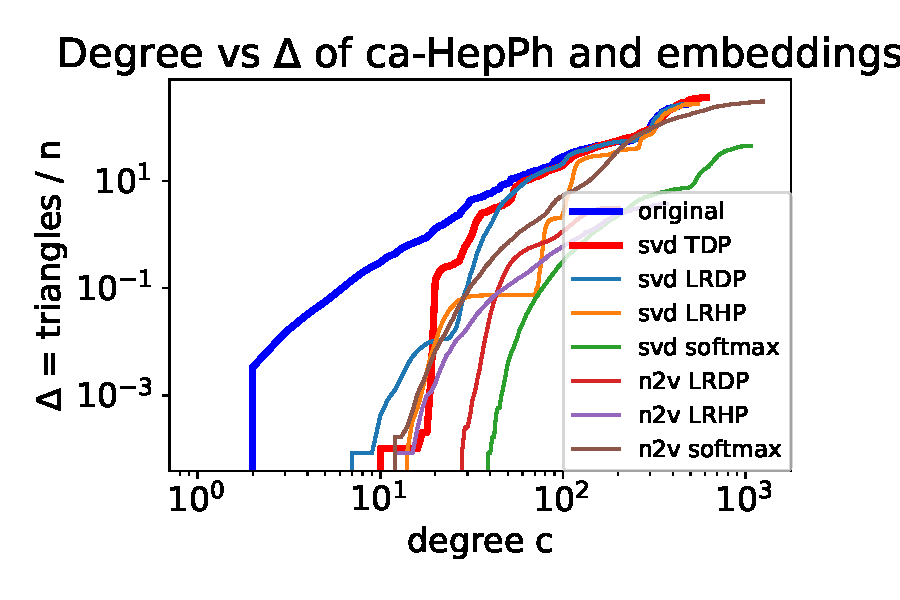
\includegraphics[scale=.35]{submissions/Seshadri2023/figures/ca-HepPh_tri_distro.pdf}
        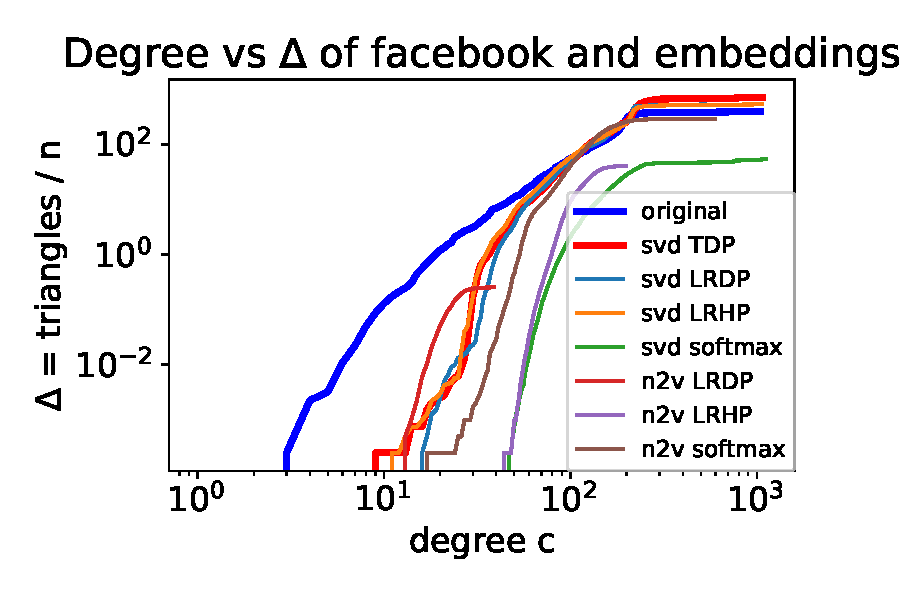
\includegraphics[scale=.35]{submissions/Seshadri2023/figures/facebook_tri_distro.pdf}
        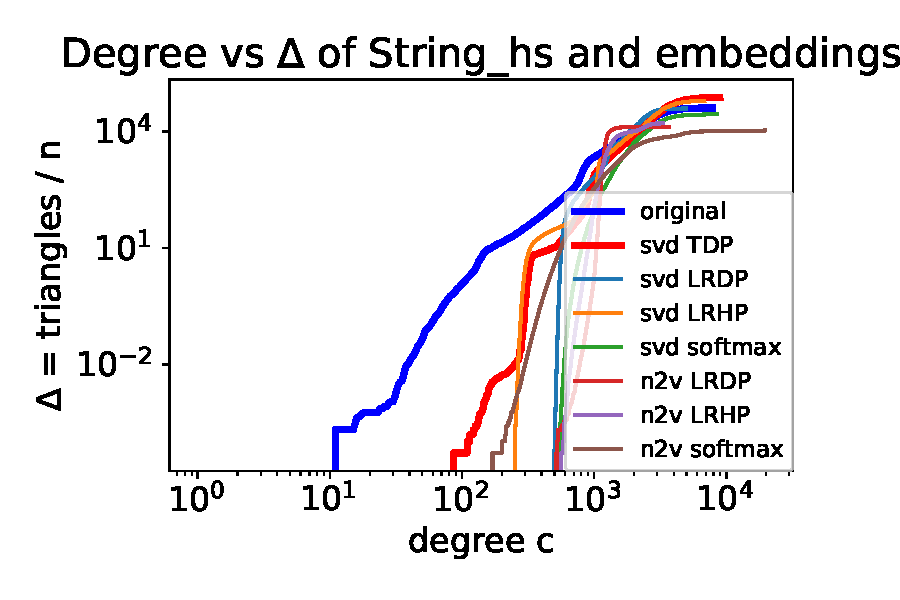
\includegraphics[scale=.35]{submissions/Seshadri2023/figures/String_hs_tri_distro.pdf} 
%         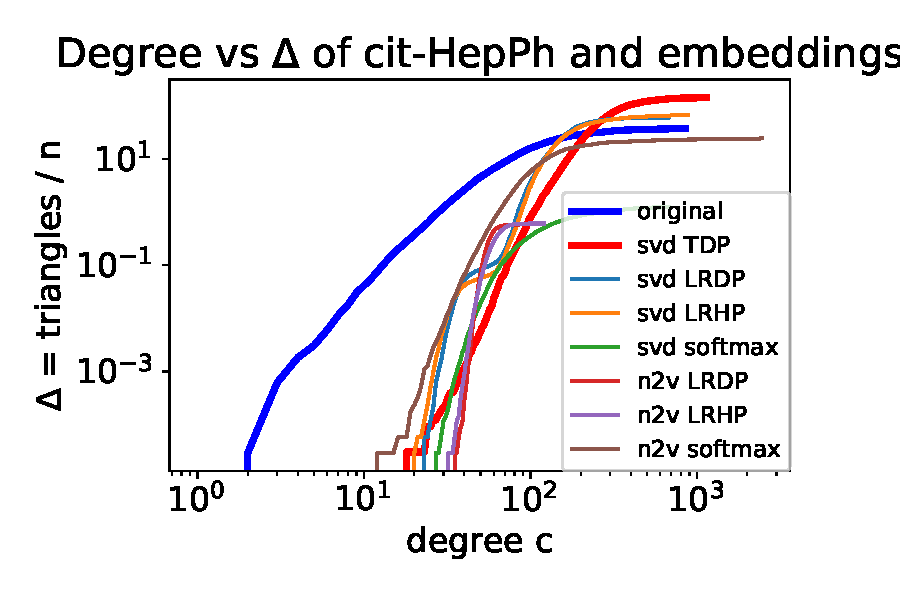
\includegraphics[scale=.37]{submissions/Seshadri2023/figures/cit-HepPh_tri_distro.pdf}
				\captionof{figure}{\small Plots of degree $c$ vs $\Delta$: We plot results for a variety
                of real-world graphs: (i) {\tt ca-HepPh}, a High Energy Physics coauthorship network (ii)
                {\tt Facebook}, a small snapshot of a Facebook social network, (iii) {\tt String\_hs}, a Protein-protein interaction network.
        We plot $c$ versus the total number of triangles only involving vertices of
        degree at most $c$. We divide the latter by the total number of vertices $n$,
        so it corresponds to $\Delta$, as in \Def{foundation}. We plot these
        both for the original graph (in thick blue), and for a variety of embeddings and kernel functions.
        For each embedding, we plot the maximum $\Delta$ in 
        a set of 100 samples from a 100-dimensional embedding. The embedding analyzed by
        \Thm{main} (TDP) is given in thick red. Observe how the embeddings generate
        graphs with very few triangles among low degree vertices. The gap in $\Delta$ for low degree is
        2-3 orders of magnitude. The other lines correspond to alternate embeddings,
        using the {\sc node2vec} vectors and/or different functions of the dot product.} \label{fig:intro-triangle-distro}
\end{figure}

Two hallmarks of real-world graphs are: (i) Sparsity: average degree is constant with respect
to $n$, and (ii) Triangle density: there are many triangles incident to low degree vertices~\cite{WaSt98,SaCaWi+10,SeKoPi12,DuPi+12}.
The large number of triangles is an important aspect of community structure. 

\begin{definition} \label{def:foundation} For parameters $c > 1$ and $\Delta > 0$, a graph $G$ with $n$ vertices
has a \emph{$(c,\Delta)$-triangle foundation} if there are at least $\Delta n$ triangles contained among vertices of degree at most $c$.
% Formally, let $S_c$ be the set of vertices of degree at most $c$. Then, the number of triangles
% in the graph induced by $S_c$ is at least $\Delta n$.
\end{definition}

Typically, we think of both $c$ and $\Delta$ as constants. 
{We emphasize that $n$ is the total number of vertices in $G$, not the number
of vertices in $S$.}
In Figure~\ref{fig:intro-triangle-distro}, we plot the value
of $c$ vs $\Delta$ as the thick blue line. (Specifically, the $y$ axis is the number of triangles divided by $n$.)
Observe that for all graphs,
for $c \in [10,50]$, we get a value of $\Delta > 1$ (in many cases $\Delta > 10$). 
As mentioned earlier, there is much work in network science showing that there are often a linear
number of triangles among low degree vertices~\cite{SeKoPi12,DuPi+12}.

Our main result is that \emph{any} embedding of graphs that generates graphs with $(c,\Delta)$-triangle foundations,
with constant $c,\Delta$, must have near linear rank. This
contradicts the belief that low-dimensional embeddings capture the structure of real-world complex networks.

\begin{theorem} \label{thm:main} Fix constant $c > 4, \Delta > 0$. Suppose the expected number of triangles 
in $G \sim \cG_V$ that only involve vertices of expected degree $c$ is at least $\Delta n$.
Then, the rank of $V$ is at least $\Omega(n/\lg^2n)$.
\end{theorem}

Equivalently, graphs generated from low-dimensional embeddings cannot contain many
triangles only on low-degree vertices. In all applications, $d$ is thought of as a constant,
or at least much smaller than $n$. On the contrary, \Thm{main} implies
that $d$ must be $\Omega(n/\lg^2n)$ to accurately model the low-degree triangle behavior.
This lower bound holds \emph{regardless} of how the vectors are constructed. 


\subsection{Empirical validation} \label{sec:emp}

% While the polynomials
% involved in Theorem~\ref{thm:main} are large,
We empirically validate the theory on a collection of complex
networks. For each real-world graph, we compute a 100-dimensional embedding through 
SVD and an important Deep Learning method, {\tt node2vec}~\cite{GrLe16}.
We generate $100$ samples of graphs from these embeddings, and compute
their $c$ vs $\Delta$ plot. This is plotted with the true $c$ vs $\Delta$ plot.
(To account for statistical variation, we plot
the \emph{maximum} value of $\Delta$ observed in the samples, over all graphs. The variation
observed was negligible.)
\Fig{intro-triangle-distro} shows such a plot for three different real-world networks.
 
In all cases, this plot is significantly off the mark at low degrees for the embedding. Around the lowest degree,
the value of $\Delta$ (for the graphs generated by the embedding) 
is 2-3 orders of magnitude smaller than the original value.
The local triangle structure is destroyed around low degree vertices.
The total number of triangles is preserved well, as shown
towards the right side of each plot. A nuanced view of the triangle
distribution, as given in \Def{foundation}, is required to see the shortcomings
of low dimensional embeddings.

We note that several other functions of dot product have been
  proposed in the literature, such as the softmax
  function~\cite{PeAlSk14,GrLe16} and linear 
models of the dot product~\cite{HaYiLe17}. \Thm{main} does not have
direct implications for such models, but our empirical validation holds for 
them as well. The embedding in Theorem~\ref{thm:main} uses the \emph{truncated
dot product} (TDP) function $max(0,\min(\vec{v}_i \cdot \vec{v}_j, 1))$ to model
edge probabilities. We construct other embeddings that compute edge probabilities
using machine learning models with the dot product and Hadamard product
as features. This subsumes linear models as given in~\cite{HaYiLe17}. 
We also consider (scaled) softmax functions, as in~\cite{PeAlSk14}, and standard
machine learning models (LRDP, LRHP). 

For each of these models, we perform the same experiment described above.
\Fig{intro-triangle-distro} also shows the plots for these other models.
Observe that \emph{none} of them capture the low-degree triangle structure,
and their $\Delta$ values are all 2-3 orders of magnitude lower than the original.  
Chanpuriya et al also validate these results on various other embedding methods~\cite{CMST20}.

\subsection{Counterpoints} \label{sec:counter}

We discuss two important results of Chanpuriya, Musco, Sotiropoulos, and Tsourakakis~\cite{CMST20,ChMu+21}.
The first result show that the rank lower bound of \Thm{main} can be circumvented
with an asymmetric embedding. They prove that one can construct \emph{two} matrices
$U, V \in \sRR^{d \times n}$ such that the graph distribution from $UV^T$ can generate
realistic triangle structure. They show that any bounded degree graph can be embedded
in this method with at most max-degree dimensions. This introduces a new technique
for graph embeddings. We note, however, that such asymmetric embeddings lose the geometric
structure of the standard embeddings. One wants geometric proximity of vectors to
represent structural closeness. For vertices $i$ and $j$, an asymmetric embedding approximates the edge probability
by $\vec{u}_i \cdot \vec{v}_j$, but the similarity of $i$ and $j$ would be measured
by looking at (say) $\vec{u}_i$ and $\vec{u}_j$. It would be interesting to incorporate similarity
in asymmetric embeddings.

Another result shows that, in some cases, community structure can be reconstructed
from {\tt DeepWalk} embeddings~\cite{ChMu+21}. This shows that some structure
is being retained by the embeddings. We note that these results mostly
focus on SBMs with a constant (at most 5) blocks, or only the largest few communities
in real data. \Thm{main} and the other results in this article focus on cases where
the number of blocks/communities is large. We believe that low-dimensional embeddings
can recover the top few communities, but fail to capture the rich structure 
of many small communities. In the next section, we discuss this point further.



\section{Challenges for community labeling using graph embeddings} \label{sec:poor-comm}

One central promise of unsupervised graph embedding methods is to
preserve network structure in the geometry.
To what extent do embedding methods capture
graph structure relevant to downstream ML tasks?

This section is based on the paper of Stolman, Levy, Seshadhri, and Sharma~\cite{StLe+22}.
We begin this discussion with the empirical results, because they
highlight the core observation. After that, we will go into the mathematical
explanations that relate to low-dimensional embeddings and factorization.

Consider the following well-defined \emph{pairwise
  community labeling} problem. Given two vertices $i$ and $j$, the
binary classification task is to determine whether they belong to the
same community. We note that this community labeling problem is an
instance of a broad range of community detection problems that have a
long history of study in the graph mining
literature~\cite{mmds_book}. 


\subsection{Empirical setup} \label{sec:comm-setup}

We use a set of real-world datasets with ground truth community labels,
an Amazon co-purchase graph of products and a DBLP citation network~\cite{YaLe12}.
We also create a synthetic Stochastic Block model, with 100K vertices,
and small blocks of size $20$ each. There is a dense graph within each block,
and a random sparse graph connecting all the blocks.

As explained earlier, the prediction task is to determine if an input pair $i, j$
of vertices belong to a community. (They may belong to multiple communities;
to make the problem simpler, we do not require any community labels to be determined.)

\begin{figure*}[h]
\begin{tabular}{c c c}
	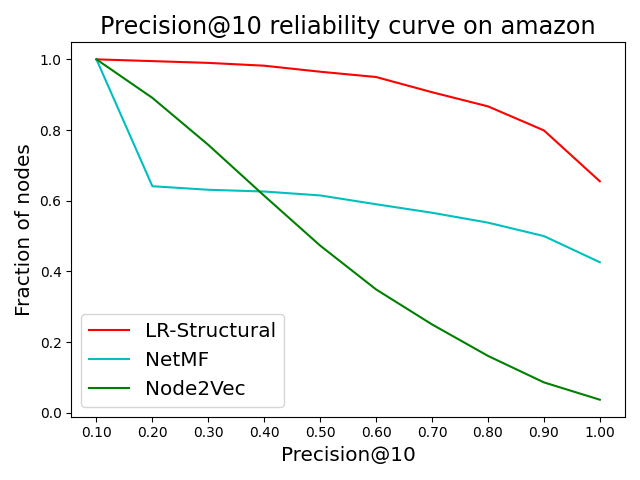
\includegraphics[width=.33\linewidth]{submissions/Seshadri2023/figures/amazon_curves.png} &
	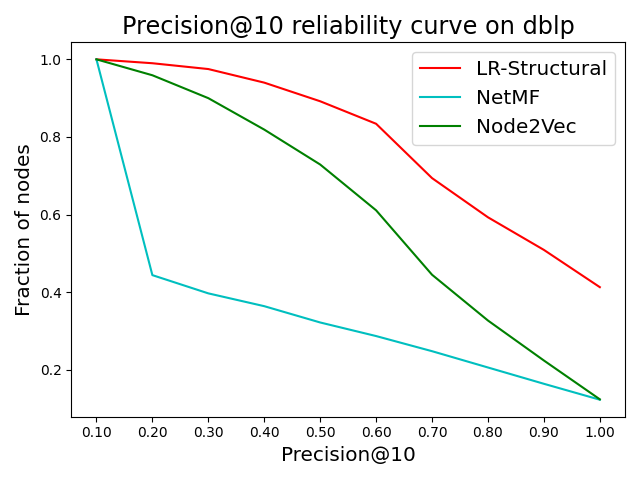
\includegraphics[width=.33\linewidth]{submissions/Seshadri2023/figures/dblp_curves.png}  &
	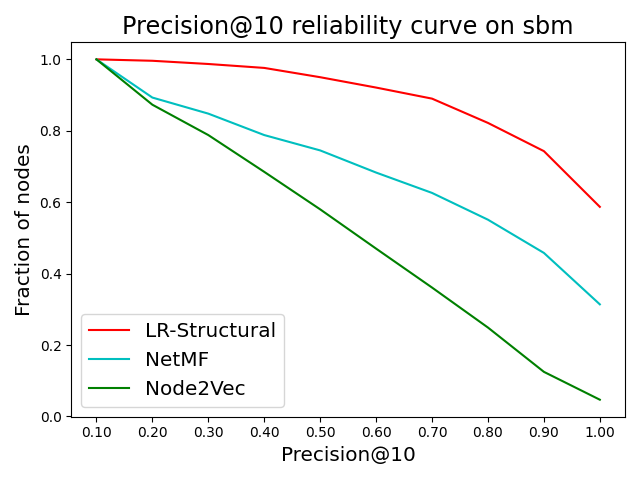
\includegraphics[width=.33\linewidth]{submissions/Seshadri2023/figures/sbm_curves.png}
\end{tabular}
\caption{Each point, $(x, y)$, on the curve represents the approximate fraction of vertices, $y$, for
	which the given method produces a precision@10 score of at least $x$. \slr is plotted against
the two best performing embedding methods. $1000$ vertices are sampled and for each vertex $v$ sampled,
the vertices of the graph
$u_1, \ldots, u_n$, are ordered by decreasing score assigned by the given classifier.
The precision@10 is the fraction of $u_1, \ldots, u_{10}$ which share a community with $v$.
Across all instances, the simple baseline $\slr$ handily outperforms more complex graph embedding methods.
}
\label{fig:p10-curves}
\end{figure*}

\paragraph{The setup for graph embeddings:} We experiment with a set of important graph
embedding methods based on factorizations and Deep Learning ({\tt{GraRep, DeepWalk, node2vec, NetMF}}~\cite{PeAlSk14,CaLu15,OuCu16,GrLe16,QiDo18}).
We note that the {\tt NetMF} method was reported to be one of the best embedding methods for node classification~\cite{GuVi+19}.
Given the embedding for each vertex, we need to construct pairwise features for pairs in $(i,j) \in V \times V$,
for the community prediction task.
The standard approach is to either take the dot product $\vec{v}_i \cdot \vec{v}_j$
or the Hadamard product $\vec{v}_i \circ \vec{v}_j$. (Recall 
that the Hadamard product is a $d$-dimensional vector whose $r$th coordinate
is the product of the $r$th coordinates of $\vec{v}_i$ and $\vec{v}_j$.)
We finally train a logistic regression model on these features for the prediction problem.
This is the standard pipeline used in prior work~\cite{covington2016deep,GrLe16,MLGSurvey20}. 

\paragraph{A simple baseline:} We compute four basic structural graph features for pairs
of vertices $(i,j)$. We look at the cosine similarity and cut size between neighborhoods, and
the Personalized PageRank values. These are well-known classic features used in the literature~\cite{SSG17,ACL07}.
We train a simple logistic regression model on these four features; the model is denoted \slr.

\paragraph{Performance metric:} For both real and simulated data, the ground truth is
sparse, i.e. the vast majority of node pairs do not belong to the same
community. We do not use AUC because of its problems in measuring
sparse data~\cite{Ha09,LiCh12}. Instead, it is appropriate to measure the prediction
performance using precision-recall curves for this highly imbalanced
label distribution~\cite{DG06}. 

The methods are evaluated by comparing the ``precision@10" distributions.
We sample 1000 random vertices. For each of 1000 vertices sampled, $v$, 
we order the other vertices of the graph, $u_1, \ldots, u_n$, in decreasing
order of their prediction score. (The model predictors based on logistic regression
on the embedding vectors or structural features assign a score in $[0,1]$.) 
We compute the precision, per vertex, of the classifier among the top 10 scores, 
with respect to the ground truth.
When the predictor is based on dot product, this is simply the top 10 neighbors
in geometric space.
In other words, we sample a vertex at random and report
the fraction of its ten nearest neighbors with which it shares a community.

We represent the distribution of values of precision@10 scores as a reliability curve. This is the curve
$(x, y)$ such that at least a $y$ fraction of vertices sampled had a precision@10 score score of at least $x$.
Higher $y$ values for a given $x$ indicate better performance.
\Fig{p10-curves} contains the curves for the best methods against the baseline (we leave out methods
with poorer performance).

\paragraph{Main observation:} Across \emph{all instances}, the baseline \slr method heavily outperforms
the more complex graph embedding methods. The performance gap for the simple Stochastic Block Model
instance is striking. The graph is practically learnable (just a collection of dense blocks with sparse connections),
but the embedding methods fail to accurately predict pairs within blocks.
For the \slr method, in all instances, at least 90\% of the vertices have a precision@10 of at least $0.5$.
This means, for at least 90\% of the vertices, at least five of the top 10 scores are in the same
community. By contrast, for the embedding methods, this fraction is less than 75\%. When looking
for a precision of more than $0.8$, the embeddings methods have less than 20\% of vertices
achieving high scores. Overall, we observe that the embeddings methods do not perform
the community labeling task well, despite the simple \slr baseline having good precision values.

\subsection{Theoretical explanation of limitations} \label{sec:theory-comm}

As explained earlier, a large variety of graph embedding methods (including
those using Deep Learning) implicitly factorize a matrix $M$
as $V^TV$. Here, $M$ denotes some matrix representing the input graph data
or the final prediction, and $V \in \sRR^{d \times n}$ is the matrix of graph embeddings.
Broadly speaking, we can
classify these methods into two categories:

\begin{asparaitem}
    \item {\bf Direct factorizations:} Here, we set $V$ as \\$\argmin_V \|V^TV - M\|_2$, where $M$ is typically
    (some power of) the graph adjacency matrix. Methods such as Graph Factorization, GraRep~\cite{CaLu15},
    and HOPE~\cite{OuCu16} would fall under this category.
    \item {\bf Softmax factorizations:} These methods factorize a stochastic matrix, such as (powers of)
    the random walk matrix. (A stochastic matrix has row sums equal to one.) Since $V^TV$ is not necessarily stochastic, these methods apply the softmax
    to generate a stochastic matrix. Notable examples are such methods are DeepWalk~\cite{PeAlSk14} and Node2vec~\cite{GrLe16}.
    Formally, consider the normalized softmax matrix $\sm(V)$ given by 
% Our aim is to show that
% embedding methods based on the softmax function must have high rank. Formally,
% the embedding method produces vectors $\vec{v}_1, \vec{v}_2, \ldots,
% \vec{v}_n$. Let $V$ denote the matrix where these vectors are columns. Methods
% like Deepwalk and node2vec model $M$ as follows. Consider the Gram matrix
% $V^TV$, and define matrix $\tM$ where
\begin{equation}
\sm(V)_{ij} = \frac{\exp(\vec{v}_i \cdot \vec{v}_j)}{\sum_k \exp(\vec{v}_i \cdot \vec{v}_k)}
\end{equation}
Note that $\sm(V)$ is stochastic by construction. 
\end{asparaitem}

The {\tt NetMF}~\cite{QiDo18} method interpolates between these categories and shows
that a number of existing methods can be expressed as factorization methods, especially
of the above forms.

% The embeddings are based
% on the Gramian (dot product) matrix $V^TV$, and thus, it is natural to
% see the extent to which the dot product predicts the community
% structure. This measures
% the ability of geometric similarity (dot product) to predict community similarity.
% We note that the dot product is commonly used in
% previous work on graph embeddings~\cite{MLGSurvey20}. 

\paragraph{The notion of community pairs:} We start with an abstraction of community structure from a matrix
standpoint: many dense
blocks in an overall sparse matrix. We quantify ``how
much" community structure can be present in a matrix $V^TV$ or
$\sm(V)$, for any matrix $V \in \sRR^{d\times n}$ (for
$d \ll n$). This formulation captures the fundamental notion of
a low-dimensional embedding, without referring to any specific method
to compute it. 

Let us start with an $n \times n$ matrix $M$ that represents the ``similarity" or likelihood of connection
between vertices. This is the final prediction matrix for community labeling. 
For convenience, let us normalize so that the $\forall i \in [n], \sum_{j \leq n} M_{i,j} \leq 1$.
(So the sum of similarities of a vertex is at most $1$.) A communities is essentially
a dense block of entries, which motivates the following definition. 
We use $\seps$ to denote a parameter for the threshold of community strength. One should think
of $\seps$ as a small constant, or something slowly decreasing in $n$ (like $1/\poly(\log n)$).

\begin{definition} \label{def:comm} A pair of vertices $(i,j)$ is a 
\emph{potential community pair}
if both $M_{ij}$ and $M_{ji}$ are at least $\seps$.
\end{definition}

Note that we do not expect all such pairs $(i,j)$ to truly be together in a community.
Hence, we only consider such a pair a potential candidate.
We expect community relationships to be mutual, even if the matrix $M$ is not. A community
can be thought of as a submatrix where at least a constant fraction of pairs are potential community
pairs. It is natural to expect
that $\Theta(n)$ pairs are community pairs; indeed, most vertices should participate
in communities, and will have at least a constant number of community neighbors. 
Our mathematical analyses shows that direct and softmax factorizations cannot produce
these many potential community pairs. 

\paragraph{Lower bound for direct factorizations:} We prove that the number
of potential community pairs in $V^TV$ is linear in the rank, and thus, a low-dimensional
factorization cannot capture community structure. The proof uses
the rotational invariance of Frobenius norms.

\begin{theorem} \label{thm:direct} Consider any matrix $V \in \sRR^{d \times n}$
such that row sums in $V^TV$ have absolute value at most $1$. Then $V$ has at most
$d/2\seps^2$ potential community pairs.
\end{theorem}

\begin{proof} \ 
Since $V^TV$ has row sums of absolute value at most $1$, the
largest absolute value of eigenvalue is also at most $1$ (a consequence of the Gershgorin circle theorem~\cite{Ger}.). 
The rank of $V^TV$ is at most $d$, so $V^TV$ has at most $d$ non-zero eigenvalues.
We can express the Frobenius norm squared, $\|V^TV\|^2_2$, by the sums of squares
of eigenvalues. By the arguments above, $\|V^TV\|^2_2 \leq d$. 

But the Frobenius norm squared $\|V^TV\|^2_2$ is also the sums of squares of entries. Each potential community pair
contributes at least $2\seps^2$ to this sum. Hence, there can be at most $d/2\seps^2$
potential community pairs.
\end{proof}

\paragraph{The instability of softmax factorizations:} 
The properties of softmax factorizations are more nuanced. Firstly, we can prove
that softmax factorizations \emph{can} represent community structure quite effectively.

\begin{restatable}{theorem}{softmaxpos}\label{thm:softmaxpos} For $d = O(\log n)$, there exists $V \in \mathbb{R}^{d \times n}$ such
that $\sm(V)_{ij}$ exhibits community structure. Specifically, for any natural number $b \leq n$,
there exists $V \in \mathbb{R}^{d \times n}$  such that $\sm(V)$ has $n/b$ blocks
of size $b$, such that all entries within blocks are at least $1/2b$.
\end{restatable}

Indeed, this covers the various SBM settings we study, and demonstrates the superiority of
softmax factorizations for modeling community structure. We note that a similar theorem,
for assymmetric factorizations, was proved in~\cite{CMST20}.

On the other hand, these factorizations are highly \emph{unstable} to small
perturbations. Indeed, with a tiny amount of noise, any community pair can be destroyed with
high probability. The noise model scales each vector with small $(1\pm\delta)$ Gaussian noise to
get the matrix $\sm(\spV{\delta})$. (The formal
definition is given in~\cite{StLe+22}.)
% 
% Formally, our noise model is as follows. Let $\delta > 0$ be a noise parameter.
% Think of the $i$th column of $V$ as the $d$-dimensional vector $\vec{v}_i$, which
% is the embedding of vertex $i$.
% For every vector $\vec{v}_i$, we generate an independent random Gaussian $X_i \sim \cN(0,\delta^2)$
% and rescale $\vec{v}_i$ as $(1+X_i)\vec{v}_i$ (formally, we rescale to $e^{X_i}\vec{v}_i$,
% to ensure that the scaling is positive).
% We denote this perturbed matrix as $\spV{\delta}$. We think of $\delta$ as a quantity going to zero, as $n$ becomes large.
% (Or, one can consider $\delta$ as a tiny constant.) 

\begin{theorem} \label{thm:perturb} Let $c$ denote some absolute positive constant.
Consider any $V \in \mathbb{R}^{d \times n}$. 
For any $\delta > c\ln(1/\seps)/\ln n$, the following holds in $\sm(\spV{\delta})$ (this
is the matrix formed by $\sm(V)$ with $\delta$ Gaussian noise). 
For at least $0.98n$ vertices $i$,
for any pair $(i,j)$, the pair is \emph{not} a potential community pair
with probability at least $0.99$.
\end{theorem}

Thus, with overwhelming probability, any community structure in $\sm(V)$ is destroyed by adding
$o(1)$ (asymptotic) noise. This is strong evidence that either noise in the input or numerical
precision in the final optimization lead to destruction of community structure.
These theorems give an explanation of the poor performance of the embeddings.

\section{Conclusion}

Instead of interpreting these limitations pessimistically, we reiterate the need for
rigorous, foundational work in graph embeddings and GNNs. 
The work in this article merely scratches the surface. The limitations
given in~\cite{SeSh20,StLe+22} might not hold for all low-dimensional embedding methods, but
they cover a large class of them. The limitations certainly hold for the most popular methods used,
and is reinforced by the empirical results. The counterpoints of~\cite{CMST20,ChMu+21}
lead to a more nuanced picture for specialized embedding methods. We need a deeper understanding
of how limitations can be avoided and how they relate to the downstream ML tasks.

The limitations
question a purely empirical approach of designing better and better embedding methods and GNNs.
As~\cite{GuVi+19} correctly point out, each method comes with many hyperparameters, so it might
be possible to tune one method to beat another and vice versa. Small improvements on some
test datasets might not reveal the complete picture. The theoretical and mathematical framework
discussed in this article provide a more rigorous basis for research. If there are fundamental
limitations from low-dimensional geometry for certain methods, we should not try to ``tune"
the problems away by experimenting with hyperparameters.

Overall, we believe that the work surveyed in this article provide an exciting new research
perspective for graph embeddings and GNNs.

\bibliographystyle{plain}
\bibliography{submissions/Seshadri2023/embeddings}

\end{document}
